\documentclass[a4paper,utf8]{article}
\usepackage[heading,fancyhdr]{ctex}
\usepackage{amsmath,amssymb,geometry,lastpage,ulem}
\usepackage{array,tabularx}
\usepackage{siunitx}
\usepackage{graphicx}
\lineskiplimit=1pt
\lineskip=3pt
\geometry{
    top=25.4mm, 
    left=25mm, 
    right=25mm, 
    bottom=25mm,
    headsep=5.9mm,
}
\ctexset{
    section = {format+=\raggedright}
}
\newcommand{\fgref}[1]{图~\ref{#1} }
\newcommand{\seqref}[1]{式~(\ref{#1})}
\newcommand{\qrange}[3]{\qtyrange[range-phrase = \text{$\sim$},range-units =single]{#1}{#2}{#3}}
\pagestyle{fancy}
\fancyhf{} \fancyhead[C]{材料科学基础实验} \fancyfoot[C]{\thepage\;/\;\pageref{LastPage}}
\begin{document}
\begin{center}
    {\mbox{}\\[7em]\zihao{2}\bfseries\songti
    材料科学基础实验预习报告}\\[34mm]
    {\zihao{-3}\bfseries\songti
    实验名称:\uline{\hfill\mbox{使用热流计法和平面热源法测量材料的热导率}\hfill} \\[2.9mm]
    学\quad 号:\uline{\makebox[25mm]{22301070}}\hfill
    姓\quad 名:\uline{\makebox[25mm]{杨雨燃}}\hfill
    班\quad 级:\uline{\makebox[25mm]{22材物}} \\[2.9mm]
    合作者:\uline{\makebox[25mm]{}}\enspace~
    桌\quad 号:\uline{\makebox[25mm]{}}\hfill\mbox{}\\[2.9mm]
    指导教师:\uline{\makebox[30mm]{艾斌}}\hfill\mbox{} \\[2.9mm]
    实验日期:\uline{\makebox[30mm]{}}\hfill\mbox{} \\[58.7mm]
    }
\end{center}
\newpage
\section*{【实验目的】}
    \begin{enumerate}
        \item 了解稳态热流计法测量材料的热导率(或导热系数)和样品的热阻的原理;
        \item 学会使用稳态热流计法测量不同材料的热导率和样品的热阻;
        \item 了解准稳态平面热源法测量材料的热导率和比热的原理;
        \item 学会用准稳态平面热源法测量材料的热导率和比热。
    \end{enumerate}
\section*{【实验原理】}%简单描述,含必要的公式和附图;
    \subsection*{1.热传导理论中的一些基本概念}
    傅立叶热传导定律指出,通过材料的热传导速率(单位时间传递的热量)与温度的梯度和热量流经的横截面积A成正比。对于均匀介质中的一维热传导,傅立叶热传导定律表示为:\par
        \begin{equation}
            q_c=-kA\frac{dT}{dx} \label{eq:1}
        \end{equation} \par
        式中,$q_c$是热传导的速率(单位:\unit{\watt}),它常常也被简称为热流,$A$是热量流经的横截面积(单位:\unit{\meter\squared}),$dT/dx$ 是温度的梯度(单位:\unit{\kelvin\metre}),比例系数 $k$ 是材料的热导率或导热系数(单位:\unit{\watt\per\meter\kelvin})。负号表示热量总是从温度高的位置流向温度低的位置。需要说明的是,傅立叶定律适用于一维稳态热传导问题。根据\seqref{eq:1},材料的热导率可写作:
        \begin{equation}
            k=\frac{q_c}{A \displaystyle \left|\frac{dT}{dx}\right|} \label{eq:2}
        \end{equation} \par
        为了引入热阻的概念,已知一块长方体匀质材料左侧的温度为 $T_1$,右侧的温度为 $T_2$,且 $T_1 > T_2$,两个侧面相距 $L$,热传导的横截面积为 $A$,假设单位时间从左侧传递到右侧的热量(即热传导的速率)为$q_c$,则材料的热阻为:
        \begin{equation}
            R_t = \frac{T_1 - T_2}{q \cdot c} 
        \end{equation}
        式中,$R_t  $为材料的热阻,它可理解为热传导速率(单位时间传递的热量)为 1W 时材料两端的
温差,它的单位为 $K/W$。如果把“热传导速率”比作“电流强度”,把“温度差”比作“电压”,
则“热阻”可比作“电阻”。就像电阻是用来表征材料对电子传输的阻碍能力,热阻的引入是
为了表征材料对热量传导的阻碍能力。\par
        \begin{equation}
            k = \frac{q_c \cdot L}{A \cdot (T_1 - T_2)} =   \cdot \frac{L}{A \cdot R_t}
        \end{equation}
        所以
        \begin{equation}
            R_t=\frac{T_1-T_2}{q_c}=\frac{1}{k}\cdot\frac{L}{A} \label{eq:3}
        \end{equation} \par

    \subsection*{2.测量材料热导率的方法简介}
        \begin{itemize}
        \item 稳态法:在样品达到稳态热传导条件下进行测量,包括保护平板法、热流计法和保护热流计法。稳态法利用傅立叶热传导定律计算热导率,计算简单,但要求样品达到稳态热传导状态,测试时间长。
        \item 瞬态法:在样品非稳态热传导条件下进行测量,包括热线法、瞬态平面热源法和激光闪光法。瞬态法测量速度快、测量范围宽,但设备复杂且昂贵。
        \end{itemize}
        \subsubsection*{3.热流计法测量材料热导率的原理}
            \fgref{fg:1} 给出了热流计法测量材料热导率的原理示意图。如图所示,加热面 A 将热量经待测样品 B 传导到散热面 C(室温)。由于加热面 A 和散热面 C 都是由热的良导体铜板制作,且与待测样品 B 紧密接触,当达到稳态时可认为其温度就是样品上、下表面的温度 $T_1$ 和 $T_2$,且 $T_1 > T_2$。对于样品 B,假设其导热方向的厚度为 $L$,面积为 $A$,当达到稳态热传导时,只要准确测量出样品的厚度 $L$ 和面积 $A$、上下表面的温度 $T_1$和 $T_2$,以及流经样品的热流 $q_c$,就可以利用\seqref{eq:3}计算材料的热导率和热阻。
            \begin{figure}[!ht]\centering
                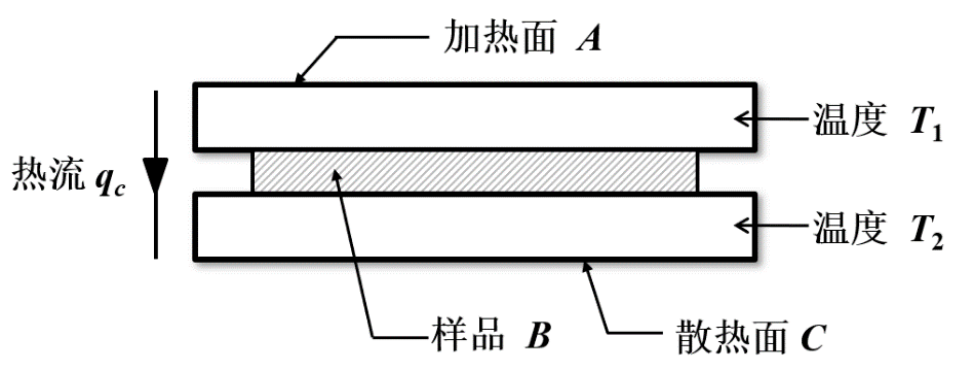
\includegraphics[width=100mm]{fg1.png}
                \caption{热流计法测量材料热导率的原理示意图 \label{fg:1}}
            \end{figure}
        \subsubsection*{4.平面热源法测量材料热导率的原理}
            如\fgref{fg:2}所示,考虑一无穷大导热平板的一维热传导问题。假设该平板的面积为无限大、厚度为 $2d$,初始温度为 $T_0$。现从平板的两侧同时向中心面施加均匀的热流密度(单位时间通过单位截面积的热量,也被称为热通量)$q_f$(\unit{\watt\per\meter\squared}),则平板上各点的温度 $T(x,t)$ 将随加热时间 $t$而变化。
            \begin{figure}[!ht]\centering
                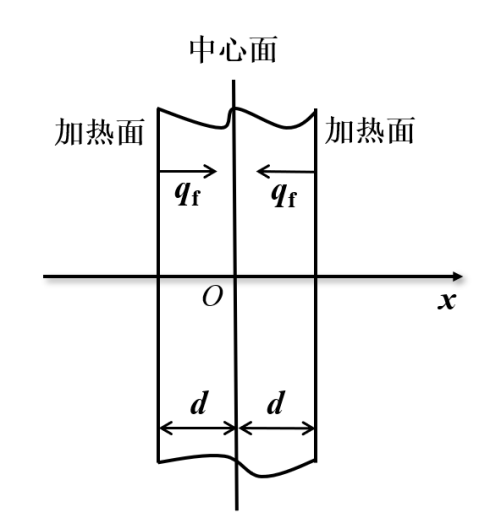
\includegraphics[width=50mm]{fg2.png}
                \caption{厚度为 $2d$ 的无穷大导热平板的一维热传导模型示意图 \label{fg:2}}
            \end{figure}\par
            以样品中心面上的一点为坐标原点 $O$,以样品厚度方向为 $x$ 轴方向,如\fgref{fg:2} 所示,则平板上各处的温度$T(x,t)$随位置 $x$和加热时间 $t$的分布可通过求解下面的偏微分方程得到:
            \begin{equation}
                \begin{cases}
                    \frac{\partial T(x,t)}{\partial t}=\alpha\frac{\partial^2T(x,t)}{\partial x^2}\\
                    \frac{\partial T(d,t)}{\partial x}=\frac{q_f}k ,\quad\frac{\partial T(0,t)}{\partial x}=0\\
                    T(x,0)=T_0
                \end{cases}
            \end{equation}
\[ \alpha = \frac{k}{\rho c} \]

其中,$\alpha$ 被称为物体的热扩散率(单位为:$\text{m}^2/\text{s}$),它是表征物体在加热或冷却的过程中升温或降温快慢的物理量。这里,$\rho$ 为材料的密度($\text{kg/m}^3$),$c$ 为材料的比热($\text{J/kg}\cdot \text{K}$),$k$ 为材料的热导率($\text{W/m}\cdot \text{K}$)。
            该偏微分方程的解说明了当热流密度$q_c$恒定时,此时加热面和中心面之间的温度差$\varDelta T$保持恒定,与加热时间 $t$ 无关,我们称这种状态为准稳态。当体系到达准稳态时:\par
            \begin{equation}
                \begin{aligned}
                    k&=\frac{q_fd}{2\Delta T}\\
                    c&=\frac{q_f}{\rho d\frac{\partial T}{\partial t}}
                \end{aligned}
            \end{equation}

\section*{【实验仪器】}%规格及参数
    DRPL-I热导率测试仪,计算机,ZKY-BRDR 型准稳态法热导率、比热测试仪,样品(石英、白橡胶、铝合金、黑橡胶、有机玻璃)。
\section*{【实验过程】}%简述主要过程和实验内容
    \begin{enumerate}
        \item 测量方块状白橡胶样品的热阻和白橡胶的热导率:1. 确保样品表面清洁,并使用丁腈手套。
        2. 使用游标卡尺测量样品的长、宽和厚度,测量五次,并记录测量结果。
        3. 将样品置于上下铜面板的中央,并固定好。
        4. 在加热器周围放置冰水混合物,确保冷却。
        5. 打开测量仪器的电源,并设置加热温度。
        6. 开始加热,直到系统进入稳态。
        7. 进行自动测量,通常需要0.5至2.5小时。
        \item 测量石柱形石英样品的热阻和石英的热导率:类似于白橡胶样品的测量过程,但需要在石英样品上下底面涂抹适量的导热硅脂以确保良好的热接触。
        \item 测量圆柱形铝合金样品的热阻和铝合金的热导率:1. 对铝合金样品进行特殊设计和制备,增加冷、热面的温差并减小横截面积。
        2. 使用绝热材料包裹侧壁,以防止热量散失。
        3. 在样品上下底面附近的侧壁上打 2 个测温孔,插入热电偶进行测温。
        4. 进行与白橡胶样品相似的测量过程。
        \item 测量有机玻璃的热导率和比热:1. 安装样品到样品架上,确保左、右横梁的安装位置正确。
        2. 预热测量仪器,设定加热电压并进行预热。
        3. 开始加热,并记录温差热电势和中心面热电势的读数。
        4. 每隔1分钟记录一次数据,确保温差热电势和中心面热电势的读数间隔均为1分钟。
        5. 一次实验最好在25分钟内完成。
        \item 测量黑橡胶的热导率和比热:1. 关闭加热开关和电源开关,取下有机玻璃样品。
        2. 重复有机玻璃样品的测量操作。
    \end{enumerate}

\end{document}